\chapter{General discussion and future directions}

\begin{remark}{Outline}

In this concluding chapter we start with highlighting some of the ongoing work, which revolves around using a promising family of priors driven by the Dirichlet process in order to model branch and site-specific parameters of codon substitution models.

Several aspects of the presented work are then put into a wider perspective, with possible extensions discussed in more detail. 

Much of the work that constitutes this thesis resolves around relaxing the standard phylogenetic assumptions, in search of more biologically plausible models. 
In that light the work on the time-heterogenous modelling, as presented in Chapter \ref{chap:epoch}, can be viewed as an introductory step towards a broader range of models that tackle different types of time-heterogeneity.
We highlight one possible extension of the epoch model, in which time changes in a non-linear fashion.
We then discuss the possibility to infer both the time and the number of change-points, or transition times, in the epoch model specification via Dirichlet process priors discussed in the first section of this summarizing chapter. 

Another substantial portion of the work presented in this thesis is devoted towards development of flexible, easy-to-use software.
%GB: perhaps better to specify more clearly what you mean with phylogenetic and population models?
In that light we talk about the continued effort to support and extend the $\pi$BUSS simulation software \citep{Bielejec2014b}, with an ever-growing array of phylogenetic and population models.

Highly dimensional estimates that result from Bayesian inference of viral spread in both time and space require dedicated software that is capable of producing visualisations that are both visually pleasing and insightful.
We discuss the future directions that the next releases of the SPREAD software \citep{Bielejec2011} will take, ensuring that it keeps providing its users with intuitive and user-friendly interfaces as well as access to a vast bulk of possible visualisations.

Finally we talk about the challenges and opportunities that the future might bring, in the era of the so-called ``genomics plenty'', where vast amount of molecular sequences can be sequenced fast and cheaply.
\end{remark}

%%%%%%%%%%%%%%%%%%%%%%%%%%%%%%%%%%%
%---DPP PRIORS FOR CODON MODELS---%
%%%%%%%%%%%%%%%%%%%%%%%%%%%%%%%%%%%
\section{Heterogenous models of codon evolution\label{sub:dpp}}

\subsection{Introduction}

The first computationally tractable models of codon substitution were independently proposed by \cite{Muse1994} and \cite{Goldman1994} and published in the same issue of Molecular Biology and Evolution (MBE).
For codon models the non-stop codon triplet $n_{1}n_{2}n_{3}$ is considered the smallest unit of evolution.
There are $4^3$ possible triplets minus three stop codons, resulting in a state space size of $61$ codons.
The standard assumption of independence is used, i.e. the substitutions at these three codon positions occur independently, and only a single change per triplet can occur at a given time. 
%GB: explain in more detail, i.e. more than 1 change is possible in subsequent infinitesimal time intervals
%GB: are there no codon models that allow for multiple substitution per time unit (I thought I recently read something like that ... will look it up and send e-mail)
Proteins are coded by a set of 20 amino acids, with each amino acid being coded by a codon triplet. 
Because there are 61 non-stop codons, inevitably some amino acids will be redundantly coded by more than 1 codon.
A substitution which does not change the encoding amino-acid is called a synonymous substitution, as it most likely leaves the protein function unchanged.
Conversely non-synonymous substitutions are more likely to affect the fitness of a particular organism.

Selective pressure is the main force behind molecular evolution.
Understanding and inferring the selective pressure is one of the central goals of molecular virology, see for example \citet{Bielejec2014a}.
That is why most of the codon substitution models are parameterized in terms of the rate of non-synonymous (denoted by convention $\beta$) and synonymous ($\alpha$ by convention) substitutions.
Their ratio $\omega=\beta / \alpha$ is a standard measure of the selective pressure \citep{ThePhylogeneticHandbook}, which is sometimes also denoted $\omega = dN/dS$.
Prevalence of synonymous substitutions over non-synonymous ones leads to a \emph{purifying (negative)} selection, and corresponds to the ratio $\omega <1$.
If non-synonymous substitutions accumulate at a faster rate than the synonymous substitutions this is coined \emph{positive selection}, improving the fitness of the particular organism.
$\omega\approx 1$ signifies neutral evolution.

There are several advantages in using codon models over nucleotide-based substitution models.
Not all DNA positions evolve at the same rate, with non-synonymous substitutions occurring more frequently then synonymous substitutions.
Although this problem can be mitigated to some extent by using codon-positioned nucleotide substitution models, the fast evolving positions and the state space limited to 4 character alphabet still can lead to biased estimates over long evolutionary distances, as portrayed in the previous Chapter~\ref{chap:pibuss}.

% GY style models
The model proposed by \cite{Goldman1994} is characterized by a substitution rate matrix with following entries:

\footnotesize{
\begin{equation}
q_{ij}^{GY94}=\begin{cases}
\pi_{j} & \text{if \ensuremath{i\rightarrow j} is a synonymous transversion}\\
\kappa\cdot\pi_{j} & \text{if \ensuremath{i\rightarrow j} is a synonymous transition}\\
\omega\cdot\pi_{j} & \text{if \ensuremath{i\rightarrow j} is a non-synonymous transversion}\\
\omega\cdot\kappa\cdot\pi_{j} & \text{if \ensuremath{i\rightarrow j} is a non-synonymous transversion}\\
0 & \text{otherwise}
\end{cases},
\label{eq:gy94}
\end{equation}
} % END: size

\noindent
where the parameter $\kappa$ denotes the transition/transversion ratio, parameter $\omega$ denotes the non-synonymous/synonymous
rate ratio and $\pi_j$ denotes the equilibrium frequency of codon triplet $j$.
The parameters $\kappa$ and $\pi_j$ can be thought of as controlling the CTMC process at the DNA level, while the $\omega$ parameter characterizes the selection on non-synonymous substitutions.
For the GY94 model the synonymous evolutionary rate is fixed to be 1, i.e. $\omega=\beta$.

Different flavours of the GY94 model differ in the composition of the equilibrium codon frequency parameter $\pi_{j}$.
One approach is to model the codon frequencies as each having the same long-time frequency of appearing. 
Such model is referred to as the GY94-Fequal.

In the GY94-F$1\times4$ model codon frequencies are calculated from the four nucleotide frequencies, with frequencies being pulled from all three codon positions, i.e. $\pi_{n_{1}}=\pi_{n_{2}}=\pi_{n_{3}}$ for all four nucleotides,.
This model leads to 3 free parameters that need to be estimated from the data. 
%GB: they're often not estimated during the MCMC run, but empirical values are used.
%GB: how are these 'nucleotide frequencies' then used to calculate the 'codon frequencies' ?
If the frequencies are parameterized according to three sets of nucleotide frequencies for the three codon positions, resulting in nine free parameters, the model is called the GY94-F$3\times4$.
Finally in the GY94-F61 model every codon triplet has it's own frequency parameter, with all parameters summing to one, resulting in 60 free parameters that need to be estimated.

The GY94-F61 model has been suggested as important in letting the model explain the data without constricting assumptions.
\citet{Rodrigue2008} however argue that the model has no interpretation on the nucleotide level as well as confounds other effects inducing uneven codon stationary probabilities.
The authors criticize the GY94-F$3\times4$ setup as superficial, pointing that the periodic pattern along the nucleotide sequence positions represents the coding structure of the sequence but not the processes that shape the evolution.

% MG style models
The Markov generator matrix for MG94 style models \citep{Muse1994} is given by:

{\tiny{
\begin{equation}
q_{ij}^{MG94}=\begin{cases}
\alpha\cdot\kappa\cdot\pi_{n}^{p} & i\rightarrow j\text{ is a synonymous transition from nucleotide \textit{m} to \ensuremath{n} at codon position \ensuremath{p}}\\
\alpha\cdot\pi_{n}^{p} & \text{synonymous transversion from \ensuremath{m} to \ensuremath{n} at position \ensuremath{p}}\\
\beta\cdot\kappa\cdot\pi_{n}^{p} & \text{non-synonymous transition from \ensuremath{m} to \ensuremath{n} at position \ensuremath{p}}\\
\beta\cdot\pi_{n}^{p} & \text{non-synonymous transversion from \ensuremath{m} to \ensuremath{n} at position \ensuremath{p}}\\
0 & \text{otherwise}
% \alpha\cdot\kappa\cdot\pi_{n}^{p} & i\rightarrow j\text{ is a synonymous transition from nucleotide \textit{m} to \ensuremath{n} at codon position \ensuremath{p}.}\\
% \alpha\cdot\pi_{n}^{p} & i\rightarrow j\text{ is a synonymous transversion from nucleotide \ensuremath{m} to \ensuremath{n} at codon position \ensuremath{p}.}\\
% \beta\cdot\kappa\cdot\pi_{n}^{p} & i\rightarrow j\text{ is a non-synonymous transition from nucleotide \ensuremath{m} to \ensuremath{n} at codon position \ensuremath{p}.}\\
% \beta\cdot\pi_{n}^{p} & i\rightarrow j\text{ is a non-synonymous transversion from nucleotide \ensuremath{m} to \ensuremath{n} at codon position \ensuremath{p}.}\\
% 0 & \text{otherwise.}
\end{cases},
\label{eq:mg94}
\end{equation}
} % END: size
}

There are two main differences to be noted with respect to the GY94 style codon models.
First, the model is parameterized in terms of both the non-synonymous ($\beta$) and synonymous ($\alpha$) rates, meaning that a change in the ratio may be due to alteration of the rate of non-synonymous or synonymous substitutions, or both.
Second, the model estimates the frequencies of the target nucleotide $\pi_{n}^{p}$ rather than of the target codon triplet $\pi_{j}$, as in the GY94 model.
As before the MG94 model can be used with frequencies specified as a single (MG94-F$1\times4$) or three (MG94-F$3\times4$) vectors with 4 dimensions.
For the remainder of this chapter we will focus our estimation on the MG94 parameterization, mostly because the parameterization in terms of both the synonymous and non-synonymous substitution rates offers interesting opportunities for disentangling the patterns of correlation between the two.

% first talk about across site variation
%GB: when you say constant, do you mean homogeneous?
Molecular phylogenetic analyses using codon models are typically restricted to fitting a single model, with constant parameterization across data, i.e. sites of the alignment.
However there is no biological reason to assume that all the sites are under the same selection regime.
\cite{NY98} point towards the fact that for most real world data sets, of which we know that they evolved under positive selection pressure only a handful of sites actually contributed towards the non-synonymous to synonymous rates ratio >1.
%GB: replace constant with homogeneous?
Therefore, applying constant model to the data, without accounting for across-data heterogeneity, biases the estimates of $dN/dS$ ratio towards lower values.
In some cases this might lead to a failure in detecting positive selection even if it's actually present in the data.  
In that respect \cite{NY98} propose two models in the GY94 context, with a fixed number of categories to which a particular site can belong.
Their \emph{neutral model} assumes a category for sites where the non-synonymous mutations are neutral ($\omega_1=1$) and a category for sites which are conserved ($\omega_2=0$).
Their \emph{positive selection model} adds an extra category of positively selected sites ($\omega_3>1$).
\cite{Goode2008} employ this setup and further extend it by allowing for a change in $\omega$ parameter value at some specified time between the most-recent common ancestor and the most recent sampling time.

These models, although undeniably a step in the right direction, still make strong assumptions, among which partitioning sites into a fixed number of rate classes and estimating the rate for each class separately is probably the most restrictive one.
Ideally, the model should let the data decide how many rate classes there are, and what the site-specific values are.

A first modelling approach that comes to mind is to fit a different rate to each site in the alignment \citep{Nielsen1997}.
Although this approach might seem naive at first, it bears a valuable property in that no explicit assumption in the distribution of rates across sites is being made.
However other negative factors still persist, precluding such a class of methods from being generally applicable.
The main problem is that, particularly for long sequences, many parameters need to be estimated, increasing the computational costs.
In case of shorter sequences such a method may overfit the data, leading to a significant loss of statistical power and biased estimates.
Another approach treats site-specific rates as independent draws from some common distribution, e.g. a gamma distribution \citep{Yang1993} or inverse Gaussian probability distribution \citep{Waddell1997}, sometimes with a proportion of sites allowed to remain invariable \citep{Gu1995}.
This approach allows to model the rate variation with relatively few parameters, as well as provides pooled estimates of the distribution parameters, which can in turn be compared across different data-sets.  
In many scenarios though a single parametric distribution proves too naive of an approach to capture complex patterns of rate evolution \citep{Pond2005a}.
\cite{Yang2000} proposed to model among-site substitution rate variation in codon models by employing a mixture of different distributions.
Although mathematically possible, this proved computationally too expensive to fit mixtures of continuous distributions for the parameters of interest and the authors resort to fitting discrete approximations.
Although these constraints are being actively stretched \citep{Suchard2009,Ayres2012}, averaging over a large array of distributions remains computationally intensive. 
\citet{Pond2005a} propose a simple, yet flexible model of rate variation with an integrative method to reliably estimate the fluctuating parameters.
This method proceeds by partitioning the rate distribution into a countable number of intervals, with each interval represented by some statistic.
%GB: explain this beta model thingy
Then a beta model is used to decide what intervals the underlying rate distribution is partitioned into and calculate corresponding rate class values.
This is perhaps the most flexible approach for evaluating site-specific rate variation to date, that provides a good fit to data with only a few extra parameters.

\cite{Heath2012} introduces a model which relaxes the assumption of a strict molecular clock in a way that is alternative to the Random Local Clock models (\cite{Drummond2010}, see Subsection~\ref{sub:clocks}), which proceed by clustering branches on a tree which share the same rate.
In the approach proposed by \cite{Heath2012} both the number of the rate classes, as well as their placement are modeled using a Dirichlet process prior (DPP, \cite{Ferguson1973}). % which treats them as random variables.
Here we propose an approach which is similar in spirit to \cite{Heath2012}, although our interest lies not in modelling overall branch rates, but in modelling across-lineage heterogeneity of the parameters of codon substitution models, such as the synonymous and non-synonymous substitution rates.

Both the number and the clustering of the lineage-specific parameters are treated as random, and are controlled by a Dirichlet Process Prior.
A DPP is a "distribution over distributions" and induces clusterings with a varying number of components that can grow or shrink depending on the data and a concentration parameter.
It is thus often used as a prior over possible clusterings where the exact number and population of distinct clusters is not known beforehand.
We require no structure to be enforced on the clustering of the branches, and allow the data to drive the model in a descriptive fashion. 
Our only requirement is the prior specification of the concentration parameter of DPP, controlling whether a model prefers less clusters with many occupants or more less densely populated ones. 
By implementing our model as part of BEAST's Bayesian inference framework we allow for a hyperprior to be put on this parameter to average over all of its possible values. 
This approach avoids overparameterisation and computational overhead by achieving data-driven balance between simplicity and complexity of the model.
We use Markov chain Monte Carlo (MCMC) techniques, in which a chain with a memoryless property is constructed to draw samples from the posterior.
Although we focus our efforts on estimating the patterns of variation in codon substitution models our implementation is generally applicable to any parameters that exhibit across-data or across-time heterogeneity .
Below we describe the main aspects of the model.

\subsection{Methods}

We use a Dirichlet process prior (DPP) to model branch-specific codon parameters.
In real-world applications not every branch in the tree would display the same type of evolutonary behaviour, therefore it would be natural to expect some degree of clustering between them.
Suppose one is interested in a branch-specific parameter $\theta_{i}, i=1,\ldots,N$, where $N=2n-1$ is the number of branches in a tree with $n$ taxa. 
This parameter might be multi-dimensional, yet for simplicity our notation will be limited to the univariate case.
We expect \emph{a priori} that $K\ll N$, where $K$ denotes the number of unique clusters of branches.
All of the branch-specific parameters have the same distribution $B$:

\begin{equation}
\forall i=1,\ldots,N: \theta_{i}\sim B(\mu_{z_{i}}),
\label{eq:dpp1}
\end{equation}

\noindent
where we will use $\mathbf{z}$ to denote the vector of branch category assignments.
Each branch receives a category $z_{i},\; i\in\left\{ 1,\ldots K\right\}$, where $K\in\left\{ 1,\ldots,N\right\}$ denotes the a number of branch categories.
As an example let us consider a topology $\mathbf{F}$ with $N=3$ branches and a fixed number of categories $K=2$.
One possible realization of the vector of assignments would then be:

$$\mathbf{z}=\left(z(1)=1,\; z(2)=1,\; z(3)=2\right),$$ 

\noindent
meaning that branches one and two belong to the same category 1, and that the third branch belongs to the category 2.
Let us denote the uniquely realized branch-specific parameter values by $\hat{\theta_{j}}, j=1,\ldots,K$.
%GB: what do you mean when you say 'mechanistic' ? Do you mean 'deterministic' ?
A mechanistic function $f$ keeps track of the mapping between the branches and unique realizations $\hat{\theta_{j}}$:

\begin{equation}
\mu_{z_{1}},\ldots,\mu_{z_{N}}=f\left(\hat{\theta}_{1},\ldots,\hat{\theta}_{K},z_{1},\ldots z_{N}\right).
\label{eq:dpp2}
\end{equation}

\noindent
The idea behind using DP priors is to set up a kernel distribution with probability distribution function $P_{0}$ from which unique branch-specific candidate values $\hat{\theta_{j}}$ are drawn:

\begin{equation}
\forall i=1,\ldots,N\;\hat{\theta_{j}}\sim P_{0}\left(\mu\right).
\label{eq:dpp3}
\end{equation}

\noindent
Clustering indicators for each branch are sampled according to a Dirichlet process with intensity $\gamma$:

\begin{equation}
z_{1},\ldots,z_{N}\sim DP(\gamma).
\label{eq:dpp4}
\end{equation}

\noindent
By defining hyper-priors for the parameters of the kernel distribution and a concentration parameter of the DP, or alternatively fixing them to specific values, we complete the specification of the DPP:

\begin{equation}
\begin{array}{c}
\mu\sim P_{1}(\ldots)\\
\gamma\sim P_{2}(\ldots)
\end{array}.
\label{eq:dpp5}
\end{equation}

% One of them is to consider the branch-specific values as coming from a mixture of distributions
There are several possible implementations of the Dirichlet process for drawing the cluster indicators as defined in Equation \ref{eq:dpp4}. 
One of them is the so-called "stick-breaking" construction \citep{Sethuraman94}.
The draws from a DP are composed of a weighted sum of point masses $P$, summing up to 1 and giving rise to a discrete distribution.
The algorithm to generate a single draw from DP is given in Listing \ref{alg:stickBreaking}.

\begin{algorithm}[H]
\begin{center}
\begin{algorithmic}[1]
% \footnotesize{
%
\State $remainingLength \gets 1.0$;
%
\For{$\left( \text{int } j=0; \; j<K; \; j++\right)$}
%
\State $r\sim Beta\left(1,\gamma\right)$;
%
\State $P\left[j\right]=r \cdot remainingLength$;
%
\State $remainingLength=\left(1-r\right) \cdot remainingLength$;
%
\EndFor \\
%
 \textbf{return} $P$;
% }
\end{algorithmic}
\end{center}
\caption{ 
{ \footnotesize 
{\bf Constructing the Dirichlet process by stick breaking.} 
}% END: footnotesize
}
\label{alg:stickBreaking}
\end{algorithm}

Colloquially we can describe it as follows: we start with a stick of length 1 and break it randomly at point $r_{1}$ chosen by drawing one value from $\text{Beta}(1, \gamma)$ and assign $p_{1}$ to the length of the part of the stick that we just broke off.
We then recursively break other portions of the stick to obtain $p_{2}, p_{3}, \ldots$ and so forth, each time setting:

\begin{equation}
p_{i}=r_{i}\cdot\underset{j}{\overset{i-1}{\prod}}\left(1-r_{j}\right).
\label{eq:sticks}
\end{equation}

\noindent
Parameter $\gamma$ controls the clustering behaviour of the process.
Smaller values will lead to fewer, yet more populated categories; larger values will result in more categories being occupied by less branches.

Under our DPP model both the number of categories $K$ and category assignments $z_{i}$ are random variables, controlled by a DPP with a concentration parameter $\gamma$ and a base distribution given by $P_{0}$.
The complete likelihood of the model can be written down as:

\begin{equation}
L(\mathbf{z},K|\gamma,N,\hat{\theta_{1}},\ldots,\hat{\theta_{K}})=\gamma^{K}\cdot\frac{\underset{j=1}{\overset{K}{\prod}}\left(\eta_{j}-1\right)!}{\underset{i=1}{\overset{N}{\prod}}\left(\gamma+i-1\right)}\cdot\underset{j=1}{\overset{K}{\prod}}P_{0}\left(\hat{\theta_{j}}\right)^{\eta_{j}},
\label{eq:dppLike} 
\end{equation} 

\noindent 
where $\eta_{k}$ denotes the number of sites assigned to category $k$.
%GB: do you want to talk about the increased computational demands of codon models? and how this can be alleviated by using BEAGLE on GPUs?
%GB: do you w  ant to show a figure that explains the redundancy of the genetic code?

\subsection{Summary}
% TODO: call it `Summary & Preliminary Results', show some numericla results + plots from tests on the Galaxy data

This model is currently being  implemented in the BEAST software package.
This pending implementation is currently being tested against an implementation in the JAGS software \citep{Plummer2003}, and we are using a numerical example to compare the results.

%%%%%%%%%%%%%%%%%%%%%%%%%%%%%%
%---EPOCH MODEL EXTENSIONS---%
%%%%%%%%%%%%%%%%%%%%%%%%%%%%%%
\section{Extending the Epoch model}

In Chapter \ref{chap:epoch} we presented a time-heterogeneous substitution model, for which the different types of substitution rates %of evolution
remain constant across all lineages in any given epoch, but vary between those epochs.
We have demonstrated the validity of the method using simulations, and its applicability to empirical HIV and Influenza data sets.
We have stressed that by implementing the model as part of Bayesian framework we are able to incorporate uncertainty in the tree reconstruction into our analysis, and thus avoid the need to fix the tree topology or any other evolutionary parameters.

\subsection{Approximating non-linear functions of rate change in time\label{sub:nonlinear}}

For some classes of problems the substitution rates might not vary linearly, at the defined change-points, but rather as some arbitrarily complex function of time. 
Such functions may be difficult, or computationally demanding, to fit exactly and the epoch model may offer an approximate solution to this types of problems.
Let us consider an interval $\left[0,T\right]$ and let the elements of the substitution rate matrix $\mathbf{Q}$ vary independently as an integrable function of time, such that $\mathbf{Q}=\mathbf{Q}(t),\; t\in\left[0,T\right]$. 
Finite-time transition probabilities can be then calculated as: 

\begin{equation}
\ensuremath{\mathbf{P}}(r,T)=exp\left(r\int_{0}^{T}\mathbf{Q}(t)dt\right).\label{eq:rodrigo}
\end{equation}

\noindent
\citet{Rodrigo2008} propose a numerical approximation to $\int_{0}^{T}\mathbf{Q}(t)dt$. 
By taking points $t_{0,}t_{1},\ldots t_{n}\in[0,T]$ such that $0=t_{0}<t_{1}<\ldots<t_{n}=T$ and dividing the interval $\left[0,T\right]$ into sub-intervals $\left[t_{i-1},t_{i}\right],\; i=1,\ldots n$ of length $\triangle t_{i}=t_{i}-t_{i-1}$ we have that:   

\begin{equation}
\int_{0}^{T}\mathbf{Q}(t)dt\approx\underset{i=0}{\overset{n}{\sum}}\mathbf{Q}(t_{i}^{*})\cdot\triangle t_{i},\; t_{i}^{*}\in[t_{i-1},t_{i}].\label{eq:approx}
\end{equation}

\noindent
From Equations~(\ref{eq:rodrigo}) and (\ref{eq:approx}), by the definition of the Riemannian integral we have that $\mathbf{P}(r,T)=\underset{n\rightarrow\infty}{lim}\underset{i=0}{\overset{n}{\prod}}\text{exp}\left(r\mathbf{Q}(t_{i}^{*})\cdot\triangle t_{i}\right)$, given that rate matrices $\mathbf{Q}(t_{i}^{*})$ commute 
and are closed with respect to the matrix multiplication.
\citet{Sumner2012} formalize the problem of multiplicative closure of the Markov models. 
Given those regularity conditions, we can perform a numerical approximation of any function of rate change by using the epoch time-discretization, and by partitioning the time interval into a fine grid of intervals.
Extending our Bayesian epoch model implementation to accommodate complex rate change functions could be the focus of future work when confronted with a problem that would benefit from such an approach.

\subsection{Evaluating number and placement of change-points in time}

Both problems presented in Chapter~\ref{chap:epoch}, i.e. HIV within-host evolution before and after progression time and seasonal influenza migration represent hypotheses that condition on a particular  number and placement the transition times.
There might however be a class of problems for which those change points are not known and need to be estimated.
% it remains interesting to investigate possible extensions that estimate the number and position of change points.
A first approach that comes to mind is to introduce priors on the number and locations of the transition times and integrate over all their possible values using the standard MCMC framework.
This straight-forward approach will however inflate the variance of the epoch-specific parameters and for some problems, e.g. viral diffusion between discretely sampled geographical locations where there is only one observation per taxon, the sparseness of data might be a factor impeding any accurate inference.

In Subsection \ref{sub:dpp} we talk about an interesting class of non-parametric prior distributions, the so called Dirichlet Process Priors (DPP). 
Although we mainly pursue the inference of lineage-specific parameters of codon models, it is interesting to note that the same class of priors could be used to infer the number and placement of transition-times of the epoch model.
At the time of writing this chapter we are testing these possibilities, yet exactly how accurate the inference of the transition times can be, and how we can quantify the predictive value of those covariates remains an open question for future studies.

%%%%%%%%%%%%%%
%---SPREAD---%
%%%%%%%%%%%%%%
\section{Future prospects for visualizing viral diffusion}

% Genetic and phenotypic data become useful only when we apply methods deriving insights from it, and these methods encompass statistical inference as well as visualization of its results. Visualizing estimates provides an efficient way to communicate results to the scientific community and beyond. Bayesian evolutionary inference, however, generates \textbf{high-dimensional} estimates, e.g. ancestral reconstructions of (multiple) traits on a posterior distribution of trees. When multidimensionality complicates the visualization task, dynamic, interactive visualizations may offer an attractive solution. In our case, the time scale of the evolutionary histories represents a natural dimension to explore for dynamic interactions. Interactivity can also encourage engagement and may lead to a better understanding and even appreciation of the statistical inference procedure itself. 

\paragraph{}
In Section~\ref{sub:clocks} we discussed how past evolutionary events can be estimated in real time units by using molecular clock models and either calibrating events or, in case of MEPs, samples obtained at various points in time.
A natural representation of this temporal dimension is to animate the geophylogeny as it unfolds through time and space.
The visualisation of spatiotemporal history, with the possibility to dynamically examine how the diffusion process unfolds, has been the main motivation for the development of SPREAD \citep{Bielejec2011}, presented in Chapter~\ref{chap:spread}.
SPREAD allows for visualising animated geophylogenies in an automated manner, by producing it's output in time-annotated Keyhole Markup Language (KML), an ISO standard geographic markup language managed by the Open Geospatial Consortium that is read and written by most spatial software. 
KML encoding allows for manipulating virtually all aspects of mapping, colour and line thicknesses, time animation, height and placement, projection used, labelling and many more.
SPREADs GUI gives user a control over fine-tuning these parameters and the output can be used in virtual globe software like Google Earth (\url{http://www.google.com/earth/}) or high-end GIS software like ArcGIS, Cartographica.
Here we take the opportunity to discuss the design and future directions of SPREAD in more details.

\subsection{Past and current efforts in visualising phylogeography}

Geophylogenies, or more generally geo-trees are spatially referenced phylogenies, for which taxa exist in a real space and can be displayed as cartographic elements within a map \citep{Kidd2010}.   
Possibly the first diagram like that, depicting evolutionary tree over geographical map is the famous \textit{Hypothetical Sketch of the Monophyletic Origin and the Extension of the 12 Races of Man from Lemuria over the Earth} shown in \cite{Haeckel1876} (see Figure~\ref{fig:lemuria})

\begin{figure}[H]
\centering
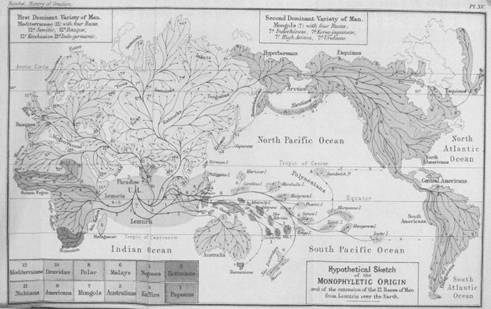
\includegraphics[scale=0.25]{lemuria}
\caption{
{ \footnotesize 
{\bf Hypothetical Sketch of the Monophyletic Origin and the Extension of the 12 Races of Man from Lemuria over the Earth.} 
} % END: footnotesize
}
\label{fig:lemuria}
\end{figure}

Ernst Haeckel, a XIX century darwinist entertained the idea that the abscence of missing fossil links in human evolution could be explained by existence of \textit{Lemuria}, a sunken land.  
The phylogentic visualisation has surpassed the, entirely discredited, work itself.

% other tools
The joint study of diffusion processes happening in geographical coordinates along with the patterns of genomic ancestry is known as phylogeography.
Summarising the findings in a clear and concise way, that can then be presented to a wider audience, is as important of a step as the statistical analysis itself \citep{Hadley2010}.
This is especially true for complex patterns of biogeographic processes, where visualisation is the key for understanding them. 
Recently great research effort has been made to visulize the phylogenetic relationships between organisms and samples in relation to their geographic distribution. 

\paragraph{}
In the first approach geographic pattern is displayed as an annotation on the tree, with branches labelled according to the names of places in which their tips are observed.
This can be carried out by hand for example in FigTree (\url{http://tree.bio.ed.ac.uk/software/figtree/}).
More advanced annotations can be achieved in iTOL \citep{itol}, which is capable of displaying charts on the internal or external branches, displaying prevalence of any kind of data, including discrete geographic locations and scaled to reflect the size of it.
This approach is most appropriate when the geographic complexity is low, as it simplifies the spatial context to text or symbolic representation, prioritising the ancestral relationship rather over the diffusion in actual geographical coordinates.

\paragraph{}
GenGis software (Figure~\ref{fig:tanglemaps}), presented by \cite{Parks2009} can, among other, generate visualisation which are an example of so-called tangle-maps.
Tangle-maps are visualisations which combine cartographic maps with images of trees.

\begin{figure}[H]
\centering
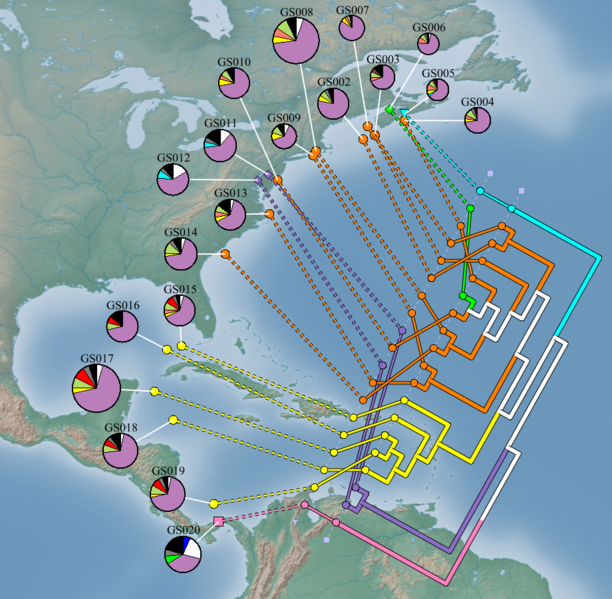
\includegraphics[scale=0.3]{tanglemaps}
\caption{
{ \footnotesize 
{\bf Tangle-map of the biodiveristy of 19 marine metagenomes.} 
Figure is plotted using GenGis (\url{http://kiwi.cs.dal.ca/GenGIS/Main_Page}).
} % END: footnotesize
}
\label{fig:tanglemaps}
\end{figure}

Although in tangle-maps the tree and the map may are visually linked through the use of graphic lines, the tree is merely overlayed on the map, rather than projected onto the geographical coordinates.

% how we do it
\paragraph{}
Model-based approaches to phylogenetic reconstruction, such as ancestral state reconstruction (see Subsection~\ref{sub:phylogeo}) provide estimates for phylogeographic relationships, but also the uncertainty in those estimates, which is crucial for hypothesis testing.
Appropriately accommodating statistical uncertainty into visualisations is a major challenge.
In BEAST and other software capable of phylogeographical reconstruction the location data can be modeled either as finite and countable (discrete) states or bivariate (longitude and latitude) realizations in continuous space.
This choice is mainly dependent on the sampling scheme of the data.
Different representations of uncertainty result from each approach.
In the continuous case when bicariate coordinates are inferred for the internal nodes using a Brownian motion model, the geographic uncertainty is expressed as confidence envelopes or credible contours for each internal node.
This can be seen in Figure~\ref{fig:cont}, where a 3D-geophylogeny with credible contours for each internal node projected on the surface in the Google Earth.

\begin{figure}[H]
\centering
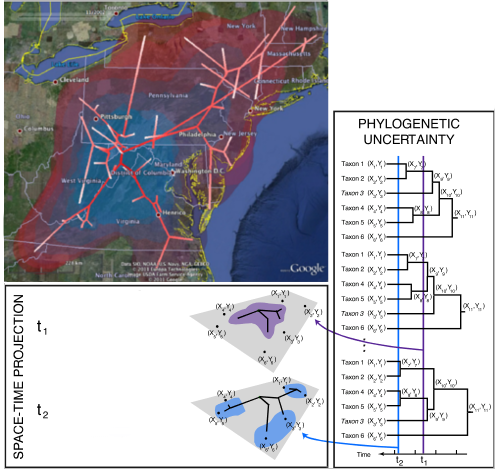
\includegraphics[scale=0.6]{continuous}
\caption{
{ \footnotesize 
{\bf Visualising geography uncertainty and phylogenetic tree uncertainty.} 
Bottom facets explain the concept of time-slicing, upper facet presents a resulting animation.
} % END: footnotesize
}
\label{fig:cont}
\end{figure}

Two time slices are shown as an example for the continuous diffusion through time. 
An example tree is mapped in continuous space, based on average bivariate coordinates for the internal nodes. 
The uncertainty at any time-slice is depicted using credible contours, obtained from slicing the complete posterior distribution of location-annotated trees, sampled by BEAST.
SPREAD supports also 2D alternatives of such projections.

\paragraph{}
In the discrete mapping , where each state represents a point location, similar easily interpreatble projections are harder to obtain.
Only branches that accommodate a state transition can be distinguished and are projected as arcs, as depicted in Figure~\ref{fig:discrete}.
This lead to a restrictive assumption of SPREADs approach, i.e. all nodes are assumed to have lived in the locations from which samples were obtained.
The circle diameter reflects the number of branches that maintain a single state according to the parent and descendent node state.

\begin{figure}[H]
\centering
\includegraphics[scale=0.4]{discrete}
\caption{
{ \footnotesize 
{\bf Phylogeographic visualization of viral spread in discrete space.} 
A. Conceptual representation of time-slicing a phylogeny and projecting the part of the tree up to time $t_{1}$ and $t_{2}$ respectively. 
B. An example projection of influenza H5N1 over time in Google Earth for two different segment phylogenies. % (hemagglutinin and neuraminidase in green and magenta respectively).
} % END: footnotesize
}
\label{fig:discrete}
\end{figure}

% now highlight some of the future perspectives
\subsection{Future perspectives}

With over 90 citations by the time of writing this thesis, the original manuscript presenting the SPREAD software (\citet{Bielejec2011}, see Chapter \ref{chap:spread}) indicates a clear need for a package that can visualize phylogeographic diffusion processes inferred using Bayesian methods.
With that responsibility in mind we will continue to support SPREAD by adding new functionalities and making more analyses possible.
The next major release of the software will be aimed at a thorough re-write of SPREADs internal engine, that would hopefully result in a more stable and responsive package.
% Specifically we will target many of the feature requests, for example the ability to instantenously alter line and polygon coloring without the need to re-compute the analysis.

% outputting KML and web interfaces
\paragraph{}
The ability to output time-stamped KML documents which can then be played as animations is one of the most important functionalities of SPREAD and a source of its popularity.
Future releases will continue to support that function, yet we will also add the ability to produce animated documents which can be embedded in webpages, viewed on mobile devices or locally on web browsers.
In our digital age, web visualization ensures accessibility and avoids the need to design proprietary software and plug-ins. We propose to merge data visualization concepts, interactive design and web development using D3 (\url{d3js.org}), a powerful JavaScript library for custom, web-based visualization. 
We will aim for a general visualization tool that maps the evolutionary patterns of traits with their uncertainty over time in their appropriate space. 
% For preliminary examples of interactive visualization see \url{http://justsz.github.io/pandemix/h9n2_AR.html}


%PL: provide a bit more background on these spatial stats: wavefront, dispersal rate, diffusion coefficient, how they are drawn from continuous diffusion reconstructions and what they can do in terms of comparative analyses and hypothesis testing..
%PL: you could also mention compatibility with BEAST2 and take this as an opportunity to describe the current situation of divergence in the two beast versions and parallel development for both.. the reader might be interested in this.
\paragraph{}
\cite{Pybus2012} introduced a conceptual link between phylogeography and spatial ecology, deminstrating that the large-scale dynamics of epidemic, traditionally estimated using time-consuming field methods, can be quantified from increasingly inexpensive molecular data.
We plan to make these new analyses attainable as part of SPREAD, with the possibility to produce spatial which can be extracted  from the posterior distribution of trees by slicing each phylogeny at multiple times and summarizing the resulting distributions.
The new release of SPREAD will also have a Command Line Interface that will make it easier to pipeline large repeatable analysis, produce scripts or call SPREAD from interpretable languages like R \citep{RCran} or Python.


%%%%%%%%%%%%%%
%---PIBUSS---%
%%%%%%%%%%%%%%
\section{Areas of improvement for the {\bussname} simulator software}

Except for empirical models of evolution, most phylogenetic methods are built on mathematical theories that predict outcomes conditional on a set of assumptions.
How well these models fit the real data, and how robust they are to the violations of these assumptions remains an open question.
Furthermore, complex biological systems targeted phylogenetic studies undergo many processes, which interact and are difficult to accurately model or distinguish from the background noise in the data.
Rapidly evolving viruses, which are the main interest of the research presented in this thesis, are subject to mutation, natural selection and spatial diffusion.
Therefore, for most of the molecular epidemiology data-sets, the true underlying evolutionary process that generated them remains unknown or particular aspects of the process remain difficult to test.
All of these factors stress the need for development of flexible simulation software, that can match the diversity, complexity and sheer amount of the real data that is currently being sampled.

% adding more models
\subsection{Model availability}

Our phylogenetic simulation software $\pi$BUSS presented in Chapter \ref{chap:pibuss} allows for fabricating evolution under a variety of coalescent, amino-acid, nucleotide and codon substitution models, as well as diffusion models, combined with various molecular clock models.
In addition it offers an ability to apply different models across arbitrary partitioning schemes. %PL: also epochs?
In future releases of $\pi$BUSS the collection of available models and data types will be extended even further.
The development effort will be aimed at matching the model richness available for inference in BEAST, and supplying every method with its simulation counterpart in $\pi$BUSS.
Specifically we will implement simulation counterparts for the flexible coalescent priors, like skyline \citep{Drummond2005} or skyride \citep{Minin2008b}.
Various extensions of biologically realistic codon models with across-site and across-branch variation will appear in future releases of the software.

Currently simulation of trait data in $\pi$BUSS is limited to discrete univariate traits.
With a growing attention received by multivariate trait data, spurred by the growing interested in continuously sampled comparative biological data, there will arise a need simulate under processes generating such data.
We plan to implement several models to do so, such as Brownian diffusion models, relaxed random walk models and models driven by the Ornstein-Uhlenbeck process.

\subsection{Graphical user interface and BEAUti integration}

% gui for more complex models
The models' specification will continue to be available via the user-friendly Graphical User Interface (GUI), which allows to setup a simulation by choosing models from drop-down menus, partitioning data in tables and parsing parameters from text fields in an intuitive fashion.
Time-heterogenous models, for which evolutionary parameters change both across different lineages (see Subsection~\ref{sub:dpp}) as well as models of pan-lineage change (see Chapter \ref{chap:epoch}) will have dedicated panels, where users can formulate them without the need to manually edit XML files.
% beauti integration
In addition to it's Command Line Interface for scripting purposes and XML parsers available via BEAST's core implementation, $\pi$BUSS is in a sense similar to the BEAUti software package, which helps BEAST users in setting up their analysis through a user-friendly GUI.
We will proceed along that path, by providing even closer integration between the two programs and facilitating generation of joint simulation-analysis XML documents in which fabricated data is instantly passed to BEASTs XML parsers for inference.

% indel models
\subsection{Simulation of insertion deletion events}

In the field of molecular biology, insertions and deletions (indels) exist on the other end of spectrum of mutations then substitution events, which we discussed in details in Subsection \ref{sub:subst_models}.
Whereas substitutions are point mutations which replace one nucleotide with another, indels proceed by either inserting or deleting nucleotides in a sequence, thus altering its length. 
Indel mutations are well known to have a significant impact on processes of molecular evolution \citep{Fletcher2009}. 
Therefore without models of insertion/deletion sequence simulation is somewhat limited.

%PL: you could mention why indel processes are useful -- I would think this is more for evaluating alignment procedures - and take this as an opportunity to talk about statistical alignment and joint inference of alignment and phylogeny (a la Marc's Baliphy), and that it would be great to get this in BEAST, but mention the computational hindrances. I think one of Marc's disciples also showed how to integrate such approaches in codon model approaches to identify positive selection: http://people.duke.edu/~br51/branch-site-article.pdf

%bible p7

% TODO




Realistic indel simulation requires however separate stochastic models.
Standard modelling assumptions, such as those used for standard substitution models (see Subsection~\ref{sub:subst_models}), are not realistic for insertions and deletions.


Future releases of $\pi$BUSS will implement that option, starting with the stochastic Dollo model \citep{LeQuesne1974}.




















\section{Other challenges}

% high perf computin
\subsection{High performance computing}

The ever growing availability of molecular sequences produced by high-throughput sequencing yields data which is difficult to store, let alone to analyze.
This problem is dubbed the biggest challenge for the field of molecular virology. % citation %PL: probably not just virology but molecular evolution in general?

%PL: the next sentence imemediately jumps into specifics, maybe introduce HPC and a bit of its history/strategies before coming to the limitations.
Furthermore due to hardware limitations and problems with heat dissipation we are approaching the limit of how many transistors can be put into integrated circuits.
%GB: need citation for Moore's law?
An observation which came to be known as Moore's law predicted the trend in which chip performance should double roughly every 18 months.
However because of these problems serial computations on next generations of CPUs no longer yield the same increases in speed and performance.
% citation
If we want to capitalize on vast amounts of data that are available, future development of phylogenetic software should target high performance parallel devices such as GPUs \citep{Nickolls2008} or Field-programmable gate arrays (FPGA, \citet{Kuon2008}).
%PL: here's an opportunity to talk a bit more about these things (I for one don't really know what FPGA are). GPUs are really good for particular tasks, but surely they are not the holy grail of HPC either, so talk about their advantages, drawbacks and some future perspectives... Maybe also talk about BEAGLE, its current CUDA dependency, and what the prospects are here. This is stuff that David Posada might be really interested in.

% codon models
\subsection{Biologically plausible models}

Interestingly, realistic models of evolution also bring about new computational challenges.
Models with large state spaces, such as codon models discussed in Subsection~\ref{sub:dpp} are an example of such a challenge.
Fortunately recent advances in computing on GPUs \citep{Ayres2012} provide opportunities to accelerate phylogenetic inference.
However we believe that more research will be needed to mitigate the imminent computational burdens that come with novel modeling approaches and high-throughput sequencing. 
%PL: this paragraph doesn't say much. Perhaps when you put the lineage codon models with DP process priors in the discussion, you can extend on this? 

% visualisations
\subsection{Big data}
%PL this is OK as concluding paragraph in another section, but it doesn't warrant a separate subsection as 'Big data.
The advent of next generation sequencing data has lead to the generation of complete genome sequences in short time and at relatively low costs.
This, combined with high-performance computing, will allow us to analyse the data in almost real time, and by coupling molecular sequence data with geographical information, to trace the diffusion of emerging epidemics and instantly identify potential hosts and sinks as well as other factors contributing to viral spread.   


%GB: I would have expected a lot more on codon models, both from a modelling perspective as well as a computational perspective?




















